\section{Introduction}

In recent years, the computer vision field has converged on a general method for object detection, and a standard evaluation of results.
Most current state-of-the-art object detection systems consist of three tasks: proposing regions of the image, evaluating a given region for presence of an object of a given category, and post-processing the results.
In the evaluation ground truth, each object is most commonly assumed to belong to one of a fixed set of classes; its location is approximated by placing a bounding box around pixels belonging to it.
Large datasets of such human annotations are used for evaluation of detection algorithms~\cite{pascal-voc-2010}.

With few exceptions, current detection systems are not inherently multi-class.
Instead, separate detectors are trained per class; they are deployed and evaluated independently.
The evaluation of multi-class performance, if at all given, consists of averaging the per-class metrics.
Some notable papers do make multi-class detection a priority, and accordingly evaluate in a multi-class setting, where false positives can be generated both by incorrect localization and incorrect labeling.

Although some detection systems make efficiency a goal, this is not always true.
Of course, it is important not to lock research into a single detector architecture and focus only on increasing efficiency.
That said, there are applications for which performance really is time-sensitive.
In robotics, a small finite amount of processing power per unit time is all that is available for robust object detection if the robot is to usefully interact with humans.
In large-scale detection system deployments, such as for image search, results need to be obtained quickly per image as the number of images to process is large and growing.
When processing large photo collection on end-user machines for immediate consumer navigation, the same is true.

In all these cases, an acceptable answer at a reasonable time may be more valuable than the best answer given too late.
Furthermore, the value of the answer depends largely on the target application.

\begin{figure}[h!]
\center{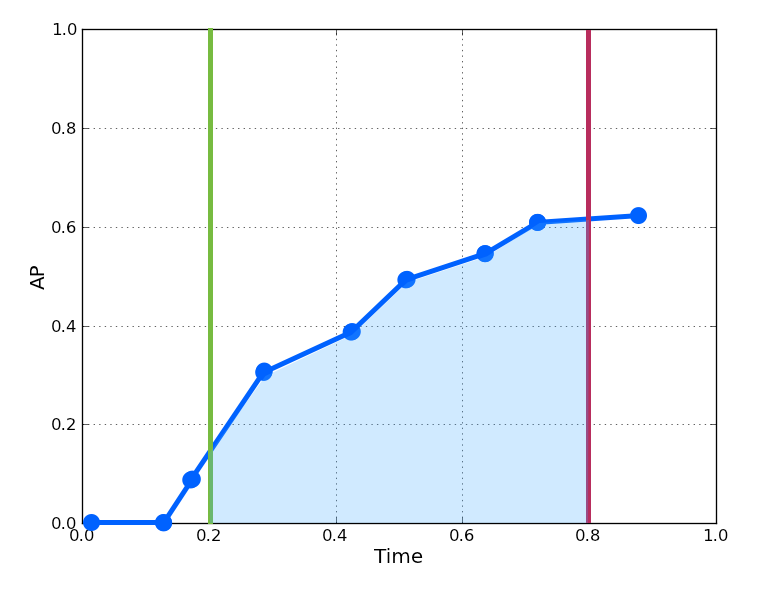
\includegraphics[width=\linewidth]
    {figures/page1.png}}
  \caption{\label{fig:page1}Our objective is to obtain Anytime performance within the bounds of the curve. That is, the policy should give the best possible answer at any given time from start time to deadline.}
\end{figure}

A hypothetical advertising system deployment presents a great case study.
A detection system will have different accuracies for objects of different classes; detections will have different values based on confidence and class; and the backlog of images will be variable in size.
The most rational detection strategy in such an environment depends on all these variables.

\subsection{Proposed Evaluation Metric}\label{sec:evaluation}
We argue that the key to tackling problems of this type is to start asking the question: What is the best performance we can get on a budget?
To answer it, we must consider the evaluation metric of performance vs. time.

Average Precision (AP) has become a standard evaluation for detector performance on challenging datasets.
This metric represents the area under the Precision vs. Recall curve, which is obtained by varying the threshold on the confidence of the detections.
The underlying measure of a correct detection is the PASCAL overlap: two bounding boxes are considered to match if they have the same label and the ratio of their intersection to their union is at least $0.5$.

Figure~\ref{fig:page1} shows our evaluation approach of plotting AP vs. time.
From the green vertical line, signifying the start time, to the red vertical line signifying the deadline, we want to obtain the best possible answer if stopped at any given time.
This corresponds to the general notion of Anytime algorithms, and is motivated by desired flexibility in the system.
Just like the metric of Average Precision itself was motivated by the inadequacy of any single Precision-Recall operating point to describe the performance of a robust system, our proposed metric is motivated by the inadequacy of any single Performance vs. Time operating point.

A single-number metric that corresponds to the stated objective is simply the area under the curve between the start and deadline bounds.

In considering ``time'' performance of detectors, none of the choices are entirely satisfying. 
Purely theoretical evaluation can hide performance inefficiencies due to computer architecture, while purely empirical evaluation depends on the low-level details of the implementation and the specifications of the hardware.
Because our multi-class detection system treats underlying detectors as ``black boxes,'' not being involed in the details of their implementation, we use basic wall clock time as our metric.

As our task is fundamentally in \emph{multi-class} object detection, we rely on a slightly different evaluation than is commonly used (although it has precedent in \cite{Desai2009}).
Instead of pooling detections across images in the dataset, and considering classes individually, we pool detections across classes, but consider images individually, reporting results averaged across the dataset.
